
%----------------------------------------------------------------------------------------
% Lecture 4: Math AD-AS (Bridge from Lecture 3 figures to equations)
% Template: SimpleDarkBlue (based on user's slide_outline.tex)
% Figures expected in ./figureAD/ :
%   figAD0.jpg figAD1.jpg figAD2.jpg
%   figAS.jpg figAS0.jpg figAS1.jpg figAS2.jpg
%   figADAS.jpg figADAS1.jpg figADAS2.jpg figADAS3.jpg figADAS4.jpg
%----------------------------------------------------------------------------------------

\documentclass[aspectratio=169,xcolor=dvipsnames]{beamer}
\usetheme{SimpleDarkBlue}

\usepackage{hyperref}
\usepackage{graphicx}
\usepackage{booktabs}
\usepackage{appendixnumberbeamer}
\usepackage{amsmath}
\usepackage{iftex}

% --- Font handling (compile anywhere) ---
\ifPDFTeX
  \usepackage[T1]{fontenc}
  \usepackage{lmodern}
  \usepackage{microtype}
\else
  \usepackage{fontspec}
  \usepackage{luatexja}
  \setmainfont{Alegreya Sans Light}[
    ItalicFont={* Italic},
    BoldFont={Alegreya Sans Medium},
    BoldItalicFont={Alegreya Sans Medium Italic}]
  \setsansfont{Alegreya Sans Light}[
    ItalicFont={* Italic},
    BoldFont={Alegreya Sans Medium},
    BoldItalicFont={Alegreya Sans Medium Italic}]
\fi

% ------------ %
% beamerbutton %
% ------------ %
\newcommand{\goto}[2]{\hyperlink{#2}{\beamergotobutton{#1}}}
\newcommand{\return}[2]{\hyperlink{#2}{\beamerreturnbutton{#1}}}
\newcommand{\extgoto}[2]{\href{#2}{\beamergotobutton{#1}}}

% --------------------------- %
% Section title page with toc %
% --------------------------- %
\setbeamertemplate{subsection page}{%
    \usebeamertemplate*{section page}
}
\setbeamertemplate{section in toc}[square]
\setbeamertemplate{subsection in toc}[square]
\AtBeginSection[]{
% \sepframe
\begin{frame}[noframenumbering]{Outline}
    % \tableofcontents[currentsection]
    \tableofcontents[currentsection, currentsubsection]
\end{frame}
}
\AtBeginSubsection[]{
  \begin{frame}[noframenumbering]{Outline}
    \tableofcontents[currentsection, currentsubsection]
  \end{frame}
}

% % ------------------------------------ %
% % Section title page with Huge bf text %
% % ------------------------------------ %
% \AtBeginSection[]{
%   \begin{frame}[noframenumbering, plain]
%     \Huge{\centerline{\textbf{\insertsection}}}
%   \end{frame}
% }

%%% automatically add spaces into enumerate and itemize environment
\let\tempone\itemize
\let\temptwo\enditemize
\renewenvironment{itemize}{\tempone\addtolength{\itemsep}{\fill}}{\temptwo}
\let\tempa\enumerate
\let\tempb\endenumerate
\renewenvironment{enumerate}{\tempa\addtolength{\itemsep}{\fill}}{\tempb}

%%=============================================================
%%  FOOTLINE TEMPLATE
%%=============================================================
\defbeamertemplate*{footline}{shadow theme}{%
    \leavevmode\hbox{%
        \hypersetup{linkcolor=white,urlcolor=white,citecolor=white}
        \begin{beamercolorbox}[wd=1.02\paperwidth, ht=2.5ex, dp=1.125ex, leftskip=.3cm plus1fil, rightskip=0.3cm]{author in head/foot}%
            \insertsectionnavigationhorizontal{.80\textwidth}{}{} \hspace{.3cm} \hfill \#\ \insertframenumber \ / \ \inserttotalframenumber%
        \end{beamercolorbox}%
    }%
}
\setbeamertemplate{footline}[shadow theme]

% --- Figures ---
\graphicspath{{../Lecture3/figureAD/}{figureAD/}{./}}

% % --- Minimal ``safe include'' helper (only used if a file is missing) ---
% \newcommand{\includegraphics}[2][]{%
%   \IfFileExists{#2}{\includegraphics[#1]{#2}}{%
%     \IfFileExists{figureAD/#2}{\includegraphics[#1]{figureAD/#2}}{%
%       \fbox{\parbox[c][0.34\textheight][c]{0.92\linewidth}{\centering\scriptsize Missing: \texttt{#2}}}%
%     }%
%   }%
% }

%----------------------------------------------------------------------------------------
%    TITLE PAGE
%----------------------------------------------------------------------------------------
\title[AD--AS (Math)]{Macroeconomics II (Spring 2026)\\\vspace{4pt}Lecture 4: AD--AS in Equations}
\author[Hui-Jun Chen]{Hui-Jun Chen}
\institute[]{National Tsing Hua University}
\date{}

\begin{document}

%------------------------------------------------
\begin{frame}[plain,noframenumbering]
    \titlepage
\end{frame}

%------------------------------------------------
\section[Dictionary]{A short dictionary: diagrams $\leftrightarrow$ equations}

%------------------------------------------------
\begin{frame}{From Lecture 3 to Lecture 4}
\begin{itemize}
\item Lecture 3: AD--AS diagrams classify shocks by \emph{comovement} of $(Y,P)$.
\item Lecture 4: write a compact set of equations that reproduces the same logic.
\item Two objects will carry almost all intuition:
\begin{itemize}
\item \textbf{Output gap} $x_t \equiv y_t - y_t^{FE}$ (tight vs slack economy)
\item \textbf{Expected price level} $p_t^e$ (what firms/households had in mind when setting wages/prices)
\end{itemize}
\end{itemize}
\end{frame}

%------------------------------------------------
\begin{frame}{Level vs rate (so we don't confuse $P$ and $\pi$ later)}
\begin{itemize}
\item \textbf{Price level:} $p_t \equiv \log P_t$.
\item \textbf{Inflation:} $\pi_t \equiv p_t - p_{t-1}$.
\item A one-time increase in $P_t$ is a level effect; persistent inflation means $\pi_t$ stays high for several periods.
\end{itemize}

\vspace{0.2em}
\begin{itemize}
\item In this lecture we keep the AD--AS vertical axis as \textbf{$P$ (or $p$)} to match the figures.
\item Next lecture we switch to \textbf{$\pi$} to study inflation dynamics explicitly.
\end{itemize}
\end{frame}

%------------------------------------------------
\begin{frame}{Output gap and unemployment (connection only)}
\begin{itemize}
\item We keep output-gap notation throughout: $x_t \equiv y_t - y_t^{FE}$.
\item Labor market tightness is often summarized by the unemployment gap:
\[
u_t - u_t^{n} \approx -\gamma \, x_t \qquad (\gamma>0)\quad \text{(Okun's law)}.
\]
\item So:
\begin{itemize}
\item $x_t>0$ (output above potential) $\Rightarrow$ unemployment below natural
\item $x_t<0$ (output below potential) $\Rightarrow$ unemployment above natural
\end{itemize}
\end{itemize}
\end{frame}

%------------------------------------------------

%------------------------------------------------

%------------------------------------------------

%------------------------------------------------
\section[RBC $\rightarrow $ IS]{RBC foundation for the IS curve}

%------------------------------------------------
\begin{frame}{Household Euler equation (RBC core)}
\small
\begin{itemize}
\item Representative household chooses $\{C_t,N_t,B_{t+1}\}$ to maximize
\[
\sum_{t=0}^\infty \beta^t u(C_t,1-N_t)
\]
subject to a budget constraint (bonds pay the real return $1+r_t$).
\item The intertemporal (bond) FOC is the Euler equation:
\[
u_C(C_t,1-N_t)=\beta(1+r_t)\,\mathbb{E}_t\big[u_C(C_{t+1},1-N_{t+1})\big].
\]
\end{itemize}
\end{frame}

%------------------------------------------------

\begin{frame}{Log utility Euler equation (no log-linearization language)}
\small
Assume \textbf{log utility} in consumption: $u(C)=\log C$, so $u_C(C)=1/C$.
The Euler equation becomes
\[
\frac{1}{C_t}=\beta(1+r_t)\,\mathbb{E}_t\left[\frac{1}{C_{t+1}}\right].
\]

\vspace{0.3em}
\begin{itemize}
\item If we ignore risk (certainty-equivalent intuition), this simplifies to
\[
\frac{C_{t+1}}{C_t}=\beta(1+r_t) \Rightarrow C_{t} = \frac{C_{t+1}}{ \beta (1 + r_{t})}.
\]
\item Higher $r_t$ raises desired consumption growth: households postpone consumption $\Rightarrow$ current demand falls.
\end{itemize}
\end{frame}

%------------------------------------------------
\begin{frame}{From the Euler intuition to a reduced-form IS}
\small
Holding expected future demand fixed, the Euler logic implies: \textbf{higher real rates reduce current demand.}
A convenient gap-form summary (setting $\sigma=1$ for log utility) is:
\[
x_t=\mathbb{E}_t x_{t+1}-(r_t-r_t^{n})+\varepsilon_t^{d}.
\]

\begin{itemize}
\item $r_t^{n}$: the ``natural'' real rate consistent with $x_t=0$.
\item $\varepsilon_t^{d}$: demand shifters (fiscal, credit, sentiment).
\item In AD--AS diagrams we often treat $\mathbb{E}_t x_{t+1}$ as roughly fixed within the period, giving a static IS.
\end{itemize}
\end{frame}

%------------------------------------------------
\begin{frame}{From Euler to an IS equation in output-gap form}
\small
Use goods-market clearing and define the output gap:
\[
x_t \equiv y_t-y_t^{FE}.
\]
In sticky-price short-run analysis, output adjusts to demand, so consumption demand translates into output demand.
Collect demand shifters into $\varepsilon_t^d$ and define the \textbf{natural real rate} $r_t^n$ as the rate that would make $x_t=0$.
A standard reduced-form IS relationship is:
\[
x_t=\mathbb{E}_t x_{t+1}-\frac{1}{\sigma}\,(r_t-r_t^n)+\varepsilon_t^d.
\]
\begin{itemize}
\item $\varepsilon_t^d$: fiscal shocks, credit conditions, confidence, preference shifts.
\item $r_t^n$: the ``RBC'' real rate consistent with potential output (no output gap).
\end{itemize}
\end{frame}

%------------------------------------------------
\begin{frame}{Static approximation used in AD--AS diagrams}
\small
In the Lecture 3 AD--AS diagrams, we effectively treat expectations terms as fixed within the period.
Holding $\mathbb{E}_t x_{t+1}$ constant gives a static IS:
\[
x_t\approx -\tilde\sigma\,(r_t-r_t^n)+\varepsilon_t^d
\qquad (\tilde\sigma>0).
\]
In levels this is the familiar linear form:
\[
Y=\bar A-a\,r,\qquad a>0.
\]
\begin{itemize}
\item This is the IS curve you plug into IS--MP to derive a downward-sloping AD.
\end{itemize}
\end{frame}


\section[AD]{Aggregate demand in equations (IS--MP $\Rightarrow$ AD)}

%------------------------------------------------
\begin{frame}{AD from IS--MP: the one mechanism}
\begin{columns}
\begin{column}{0.5\textwidth}
\centering
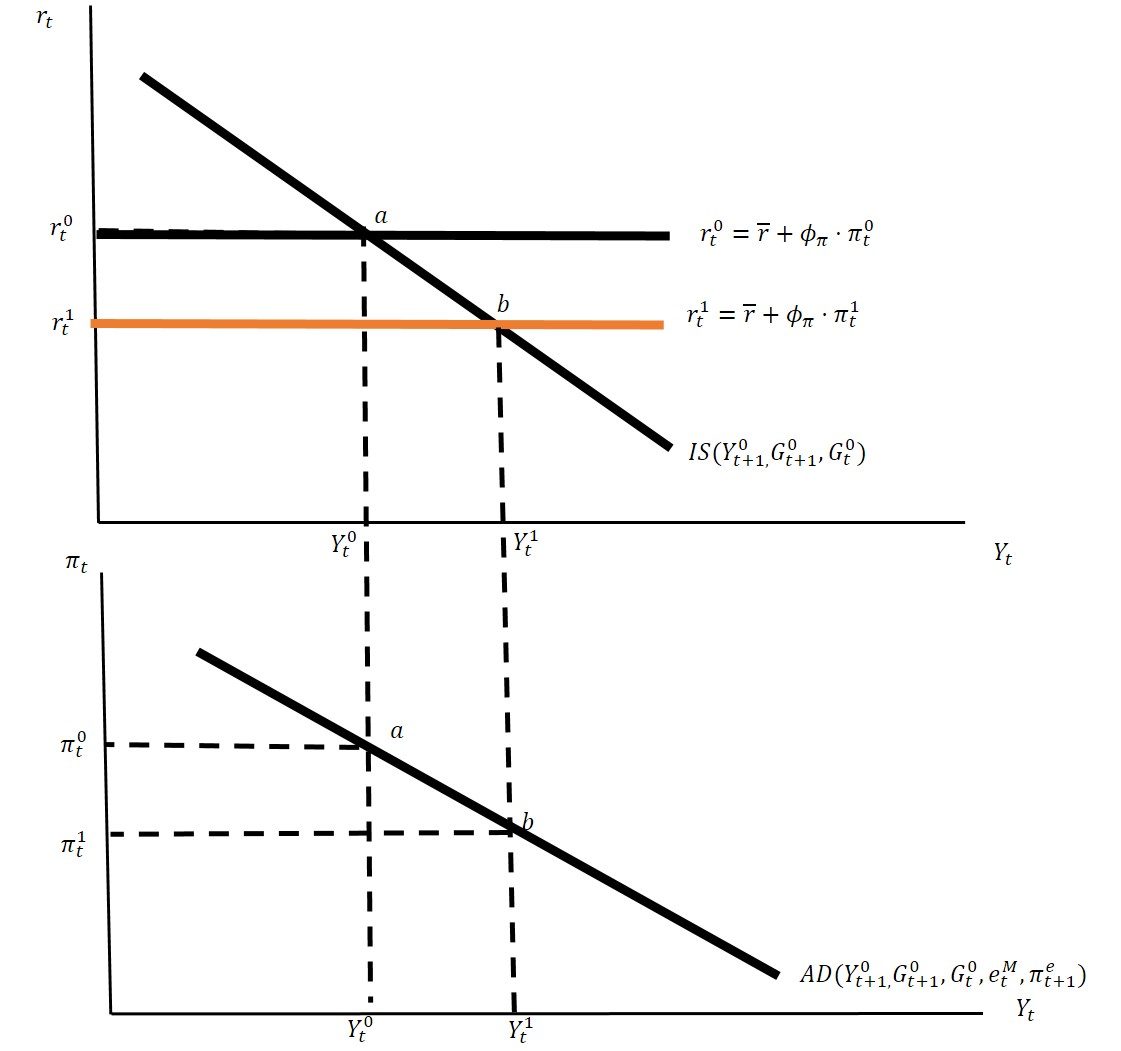
\includegraphics[width=\linewidth]{figAD0.jpg}
\end{column}
\begin{column}{0.5\textwidth}
\small
\begin{itemize}
\item Modern central banks adjust the \textbf{policy stance} in response to inflation and activity.
\item To match the figure notation, we summarize the stance with a \textbf{real} policy rate $r$.
\item Higher inflation (relative to target) $\Rightarrow$ higher $r$ under the rule.
\item Higher $r$ reduces interest-sensitive spending $\Rightarrow$ lower output.
\item Therefore higher $P$ (through higher $\pi$) is associated with lower $Y$: \textbf{AD slopes down}.
\end{itemize}
\end{column}
\end{columns}
\end{frame}

%------------------------------------------------
\begin{frame}{A simple IS--MP system (linear, with $r$ as the policy instrument)}
\small
\begin{itemize}
\item GDP Expenditure Accounting in this static model (no $I_{t}$):
\[
    Y_{t} = C_{t}(r_{t}) + G_{t}
\]
where current consumption is decreasing in $ r_{t} $, while $ G_{t} $ is fixed.
\item \textbf{IS (goods market):} output falls when the real rate rises, i.e., in a simplified form,
\[
Y = \bar{A} - a r,\qquad a>0,
\]
where $\bar{A}$ summarizes autonomous spending (preferences, $G$, taxes, etc.).
\item \textbf{MP (policy rule in real-rate form):}
\[
r = \bar{r} + \phi_{\pi}(\pi-\pi^{\ast}) + \phi_{y}(Y-Y^{FE}),
\qquad \phi_{\pi}>0,\ \phi_{y}\ge 0.
\]
\item \textbf{Link from prices to inflation:} $\pi \equiv p-p_{-1}$ with $p\equiv \log P$ and $p_{-1}$ given within period $t$.
\end{itemize}
\end{frame}

%------------------------------------------------
\begin{frame}{Solve IS + MP for $Y(\pi)$ (the AD equation)}
\small
Substitute the policy rule into IS:
\[
Y = \bar{A} - a\Big[\bar{r} + \phi_{\pi}(\pi-\pi^{\ast}) + \phi_{y}(Y-Y^{FE})\Big].
\]
Collect $Y$ terms:
\begin{align*}
(1+a\phi_{y})Y
&= \bar{A} - a\bar{r} + a\phi_{y}Y^{FE} - a\phi_{\pi}(\pi-\pi^{\ast}).
\end{align*}

\vspace{0.3em}
\begin{itemize}
\item Therefore $Y$ decreases in $\pi$: higher inflation \ $\Rightarrow$ \ higher $r$ \ $\Rightarrow$ \ lower output.
\end{itemize}
\end{frame}

%------------------------------------------------
\begin{frame}{From $Y(\pi)$ to $Y(P)$ (downward-sloping AD in $(P,Y)$)}
\small
Use $\pi = p-p_{-1}$ with $p=\log P$ and $p_{-1}$ predetermined.
From the previous slide,
\[
Y
=
\underbrace{\frac{\bar{A} - a\bar{r} + a\phi_{y}Y^{FE} + a\phi_{\pi}(p_{-1}+\pi^{\ast})}{1+a\phi_{y}}}_{\text{constant at time }t}
\;-\;\underbrace{\frac{a\phi_{\pi}}{1+a\phi_{y}}}_{\phi>0}\,p.
\]

\vspace{0.3em}
\begin{itemize}
\item Holding last period's price level $p_{-1}$ fixed, higher $p$ implies higher inflation $\pi$.
\item The policy rule reacts by raising $r$, which lowers $Y$ through IS.
\item This reproduces the \textbf{downward slope of AD} in $(P,Y)$ space without a money-supply LM curve.
\end{itemize}
\end{frame}

%------------------------------------------------
\begin{frame}{What shifts AD (in equations)}
\small
In this IS--MP derivation, AD shifts when the mapping from prices/inflation to output changes.
\begin{itemize}
\item \textbf{Demand shifters} ($\bar{A}\uparrow$): fiscal expansion, optimism, easier credit \ $\Rightarrow$ \ AD shifts right.
\item \textbf{Policy stance} ($\bar{r}\downarrow$): more accommodative rule/intercept \ $\Rightarrow$ \ AD shifts right.
\item \textbf{Potential output} ($Y^{FE}\uparrow$): raises output for given policy feedback.
\item \textbf{Rule coefficients}:
\begin{itemize}
\item larger $\phi_{\pi}$ makes AD \emph{steeper} (policy leans harder against inflation),
\item larger $\phi_{y}$ dampens the response of $Y$ to inflation (feedback through activity).
\end{itemize}
\end{itemize}
\end{frame}

%------------------------------------------------
\begin{frame}{Two textbook shifts (same pictures, IS--MP interpretation)}
\begin{columns}
\begin{column}{0.50\textwidth}
\centering
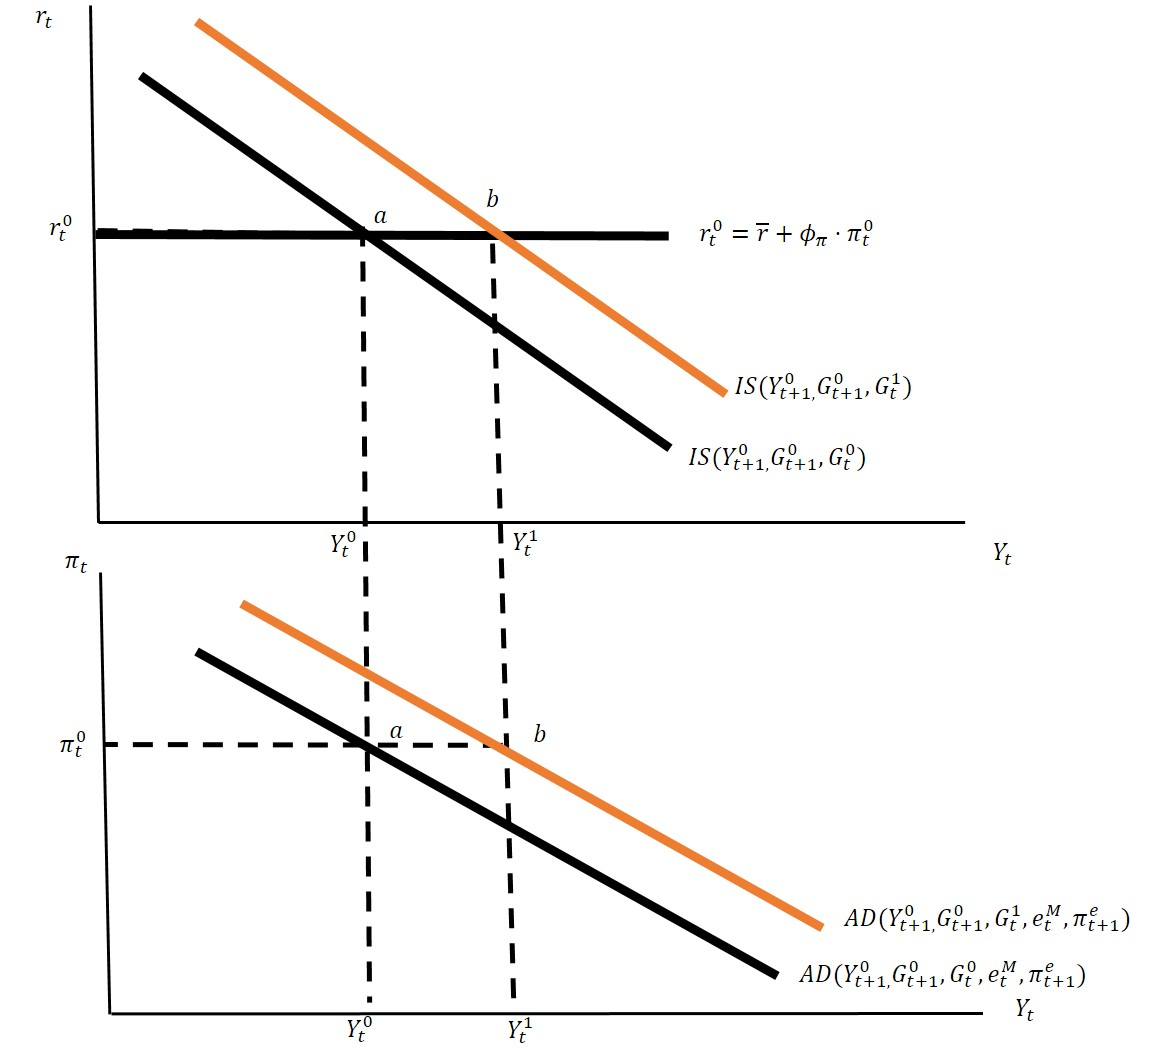
\includegraphics[width=\linewidth]{figAD1.jpg}\\[-2pt]
\small $G\uparrow$ (or $\bar{A}\uparrow$): AD shifts right
\end{column}
\begin{column}{0.50\textwidth}
\centering
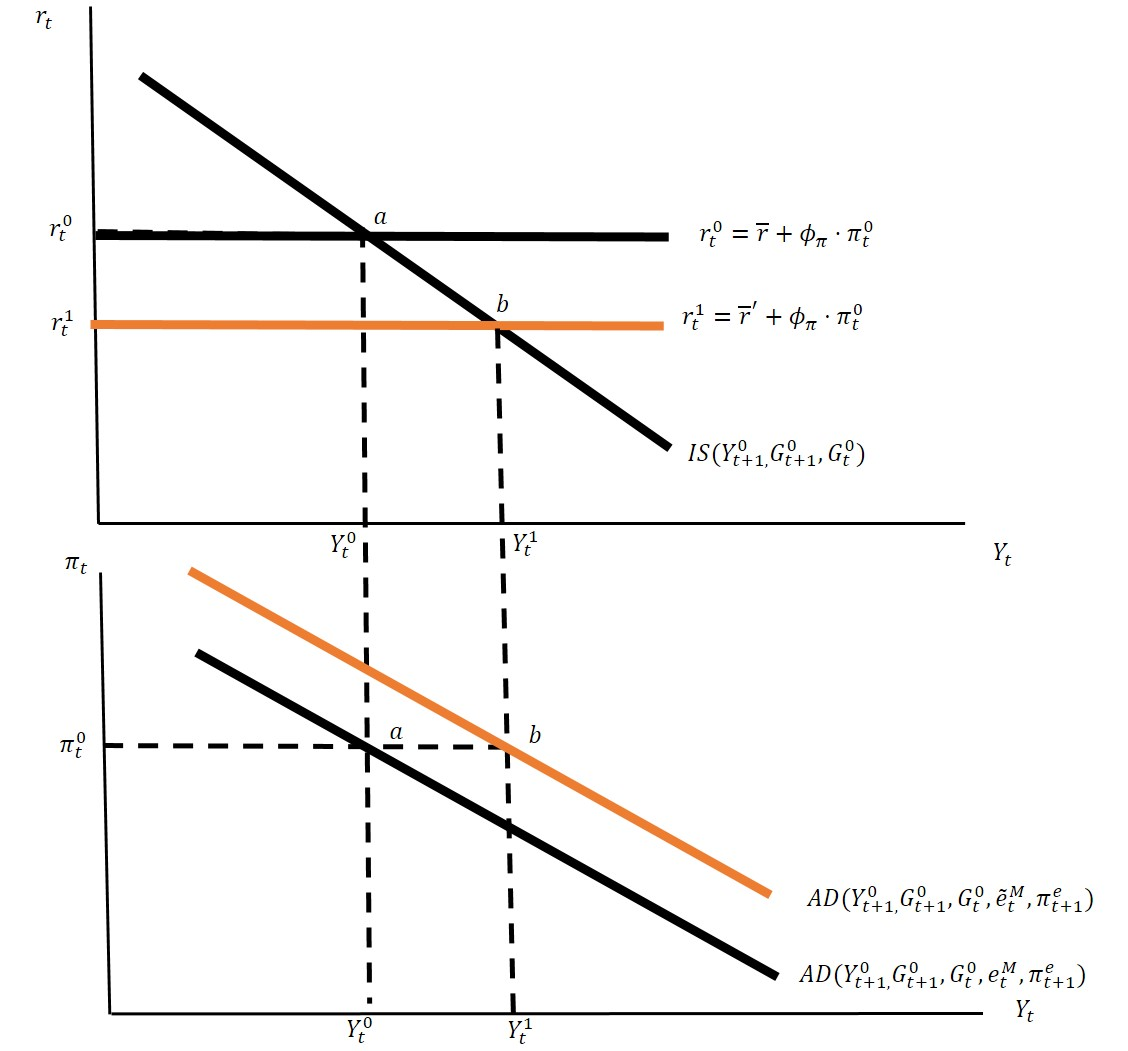
\includegraphics[width=\linewidth]{figAD2.jpg}\\[-2pt]
\small Policy easing (lower $\bar{r}$ or a more accommodative rule): AD shifts right
\end{column}
\end{columns}
\end{frame}


\section[AS]{Aggregate supply in equations (SRAS + FE)}

%------------------------------------------------
\begin{frame}{FE as the long-run supply benchmark}
\begin{columns}
\begin{column}{0.62\textwidth}
\centering
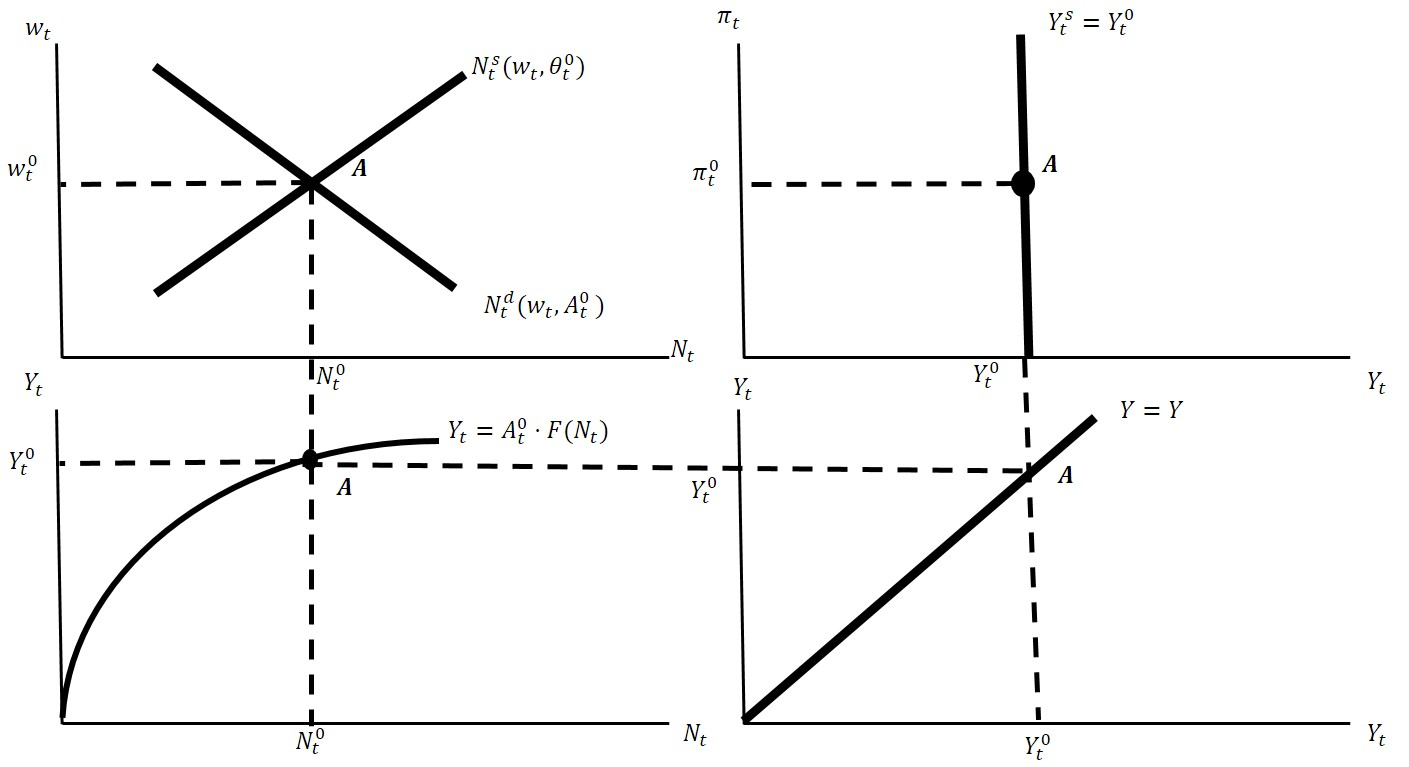
\includegraphics[width=\linewidth]{figAS0.jpg}
\end{column}
\begin{column}{0.38\textwidth}
\small
\begin{itemize}
\item FE output $Y^{FE}$ comes from the RBC supply block (labor market + production).
\item In the long run, prices adjust so output returns to $Y^{FE}$.
\item FE shifts with technology, factor supply, and capital.
\end{itemize}
\end{column}
\end{columns}
\end{frame}

%------------------------------------------------
\begin{frame}{SRAS as ``price surprises move output'' (level form)}
\small
A convenient reduced form (Lucas/expectations-augmented supply):
\[
y = y^{FE} + \alpha\,(p - p^e),\qquad \alpha>0.
\]
\begin{itemize}
\item If $p>p^e$ (prices higher than expected), real wages are lower than expected $\Rightarrow$ firms hire more $\Rightarrow$ output rises.
\item If $p<p^e$, output falls below $y^{FE}$.
\item The slope of SRAS in $(p,y)$ space is $1/\alpha$.
\end{itemize}
\end{frame}

%------------------------------------------------
\begin{frame}{SRAS written in output-gap notation}
\small
Define output gap $x \equiv y-y^{FE}$. Then
\[
x = \alpha\,(p - p^e).
\]
\begin{itemize}
\item Output gap is proportional to the \textbf{price-level surprise} $(p-p^e)$.
\item A left shift of AS in Lecture 3 corresponds to shocks that raise marginal cost for given $x$,
or (equivalently) raise the $p$ needed to produce a given $y$.
\end{itemize}

\vspace{0.3em}
\begin{itemize}
\item Next lecture we will rewrite this in inflation form and specify how $p^e$ evolves (expected inflation).
\end{itemize}
\end{frame}

%------------------------------------------------
\begin{frame}{Supply-side shifts in the figures}
\begin{columns}
\begin{column}{0.50\textwidth}
\centering
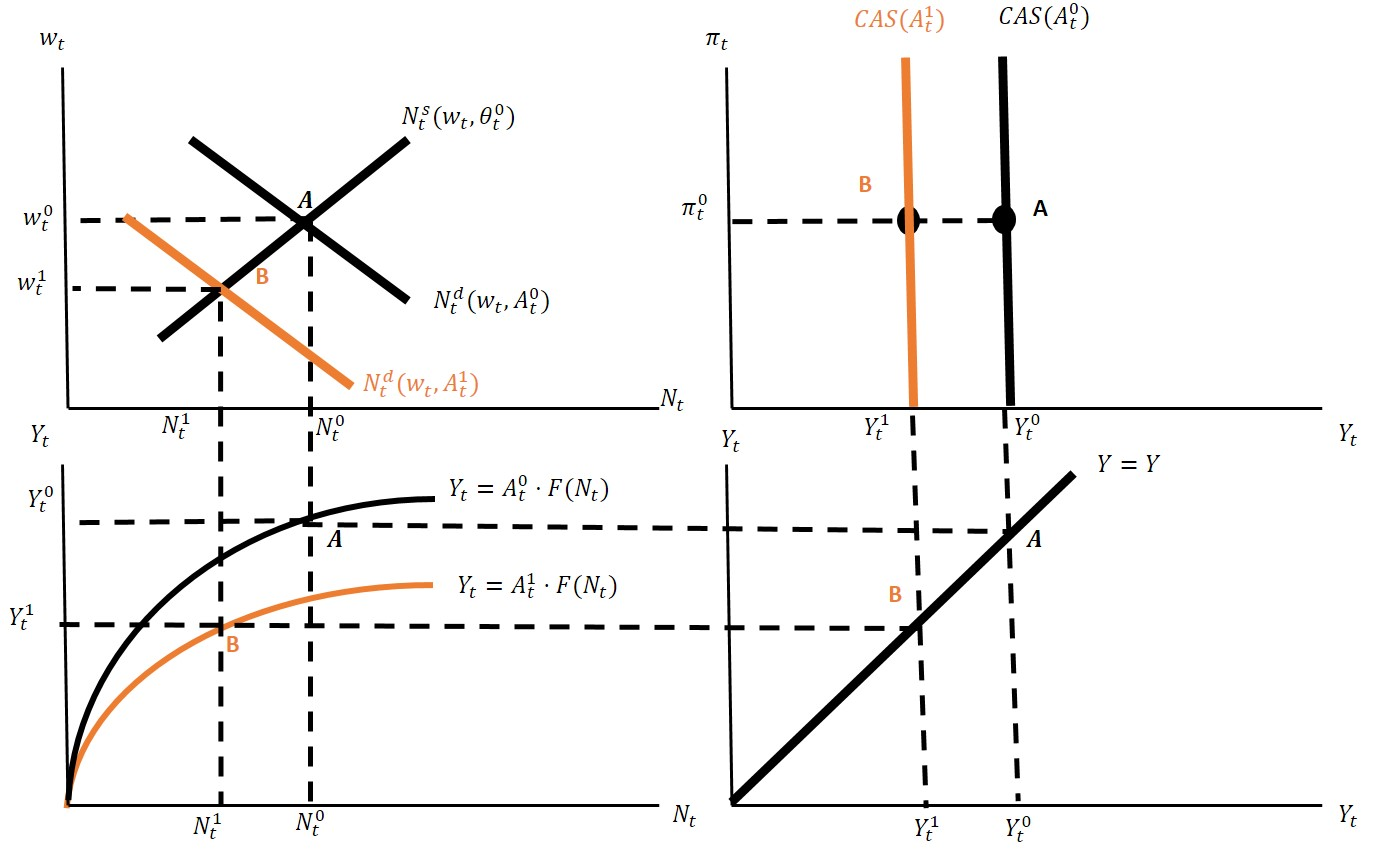
\includegraphics[width=\linewidth]{figAS1.jpg}\\[-2pt]
\small $A\downarrow$ shifts FE / CAS left
\end{column}
\begin{column}{0.50\textwidth}
\centering
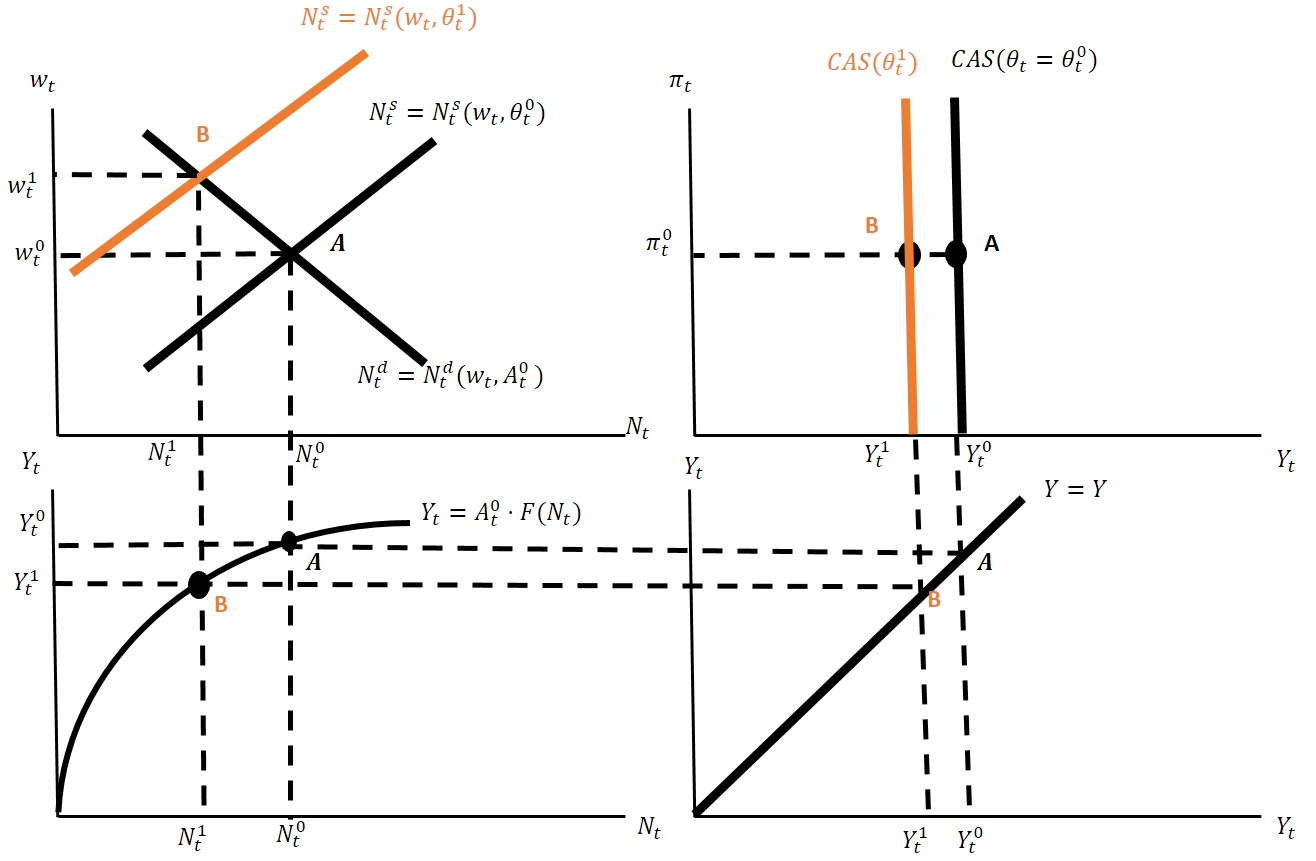
\includegraphics[width=\linewidth]{figAS2.jpg}\\[-2pt]
\small labor supply $\downarrow$ shifts FE / CAS left
\end{column}
\end{columns}
\end{frame}

%------------------------------------------------
\section[Eqn]{Equilibrium and comparative statics}

%------------------------------------------------
\begin{frame}{AD--AS equilibrium (in one picture)}
\centering
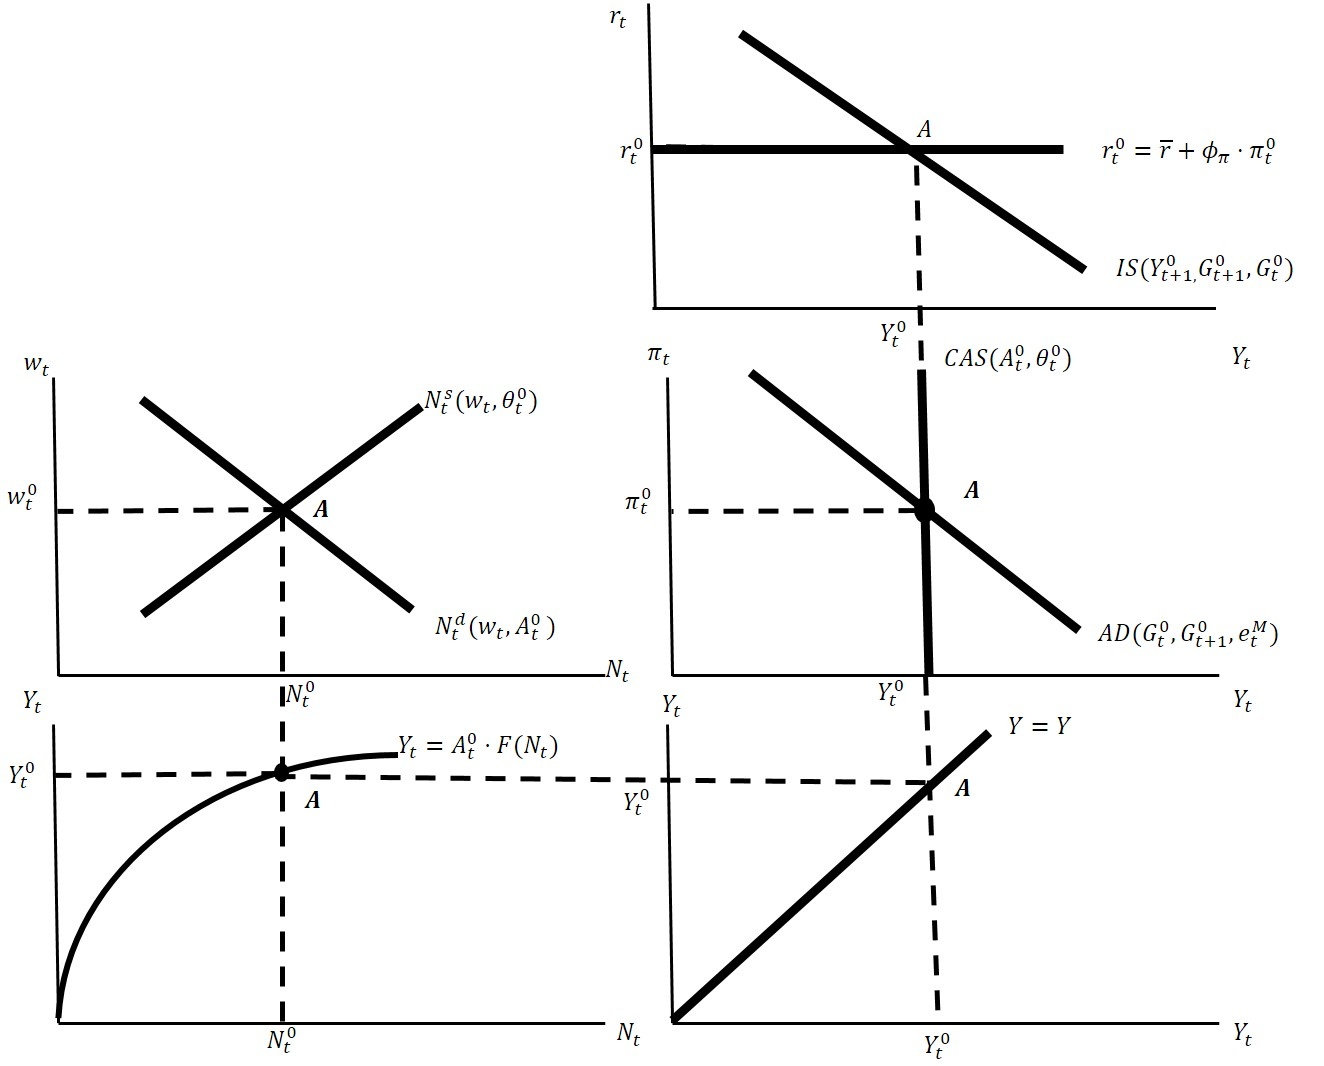
\includegraphics[width=0.65\linewidth]{figADAS.jpg}
\end{frame}

%------------------------------------------------
\begin{frame}{AD--AS equilibrium (solve once)}
\small
Use a simple AD reduced form $y = \bar{y}_D - \phi\,p$ with $\phi>0$ (downward slope), and SRAS
$p = p^e + \lambda (y-y^{FE})$ with $\lambda>0$ (upward slope).

\vspace{0.2em}
\begin{itemize}
\item Substitute AD into SRAS:
\[
p = p^e + \lambda\big(\bar{y}_D - \phi p - y^{FE}\big).
\]
\item Solve for $p$:
\[
(1+\lambda\phi)p = p^e + \lambda(\bar{y}_D - y^{FE})
\quad\Rightarrow\quad
p = \frac{p^e + \lambda(\bar{y}_D - y^{FE})}{1+\lambda\phi}.
\]
\item Then $y$ follows from AD: $y=\bar{y}_D-\phi p$.
\end{itemize}
\end{frame}

%------------------------------------------------
\begin{frame}{Demand expansion: why $(Y,P)$ move together}
\begin{columns}
\begin{column}{0.62\textwidth}
\centering
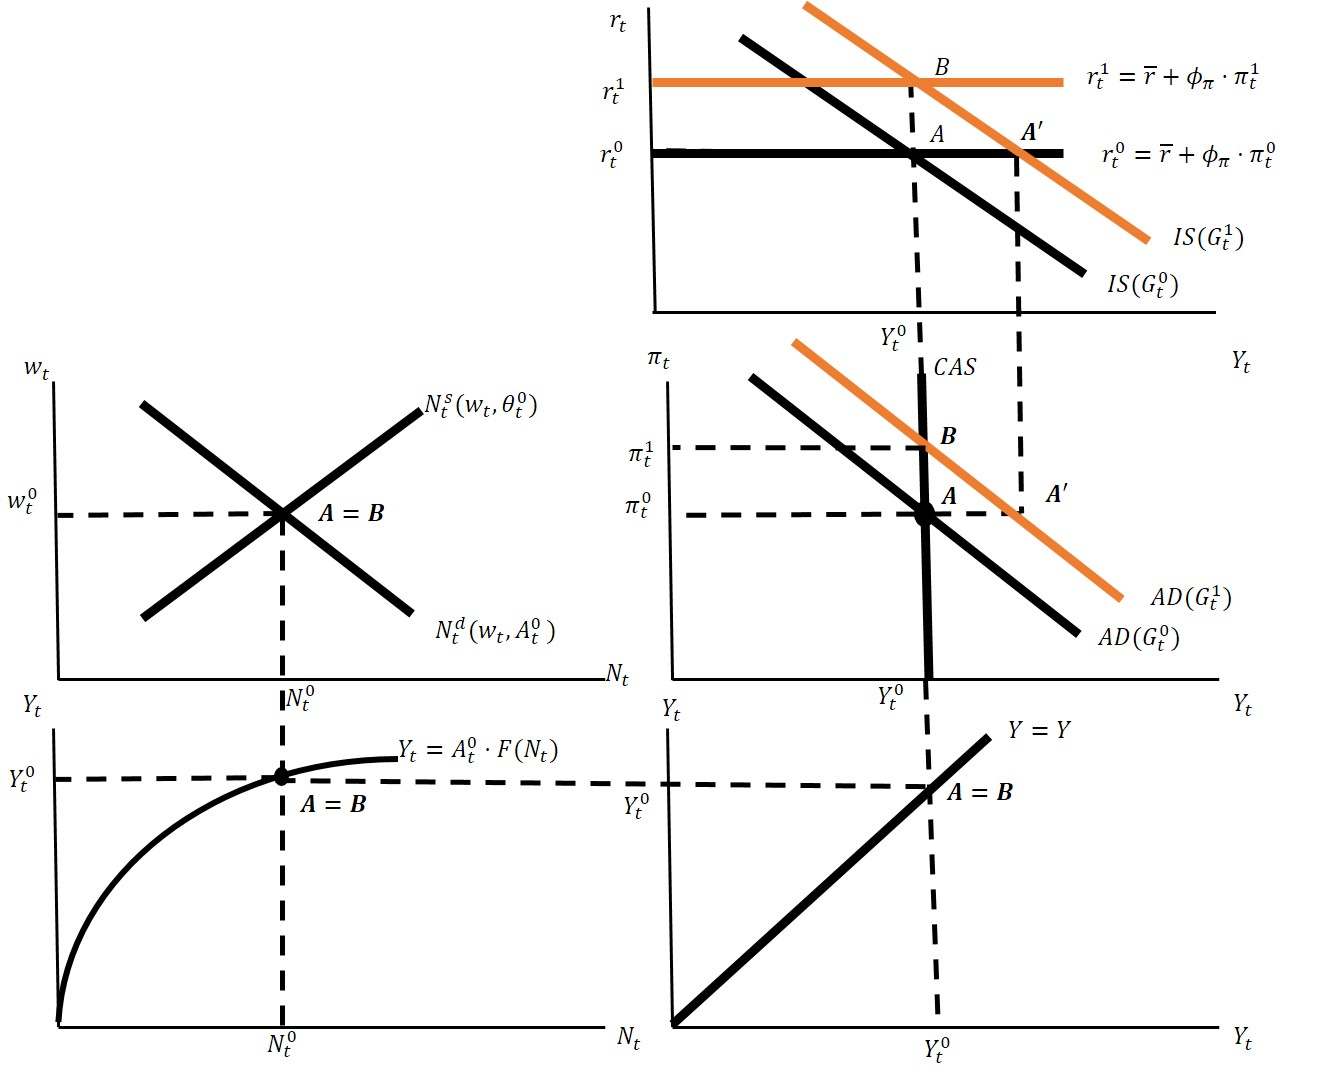
\includegraphics[width=\linewidth]{figADAS1.jpg}
\end{column}
\begin{column}{0.38\textwidth}
\small
\begin{itemize}
\item Demand expansion means $\bar{y}_D\uparrow$ (AD shifts right).
\item From the solved expression: $p$ rises when $\bar{y}_D$ rises.
\item AD then implies $y$ rises as well.
\end{itemize}
\end{column}
\end{columns}
\end{frame}

%------------------------------------------------
\begin{frame}{Monetary easing: one parameter shift, same logic}
\begin{columns}
\begin{column}{0.62\textwidth}
\centering
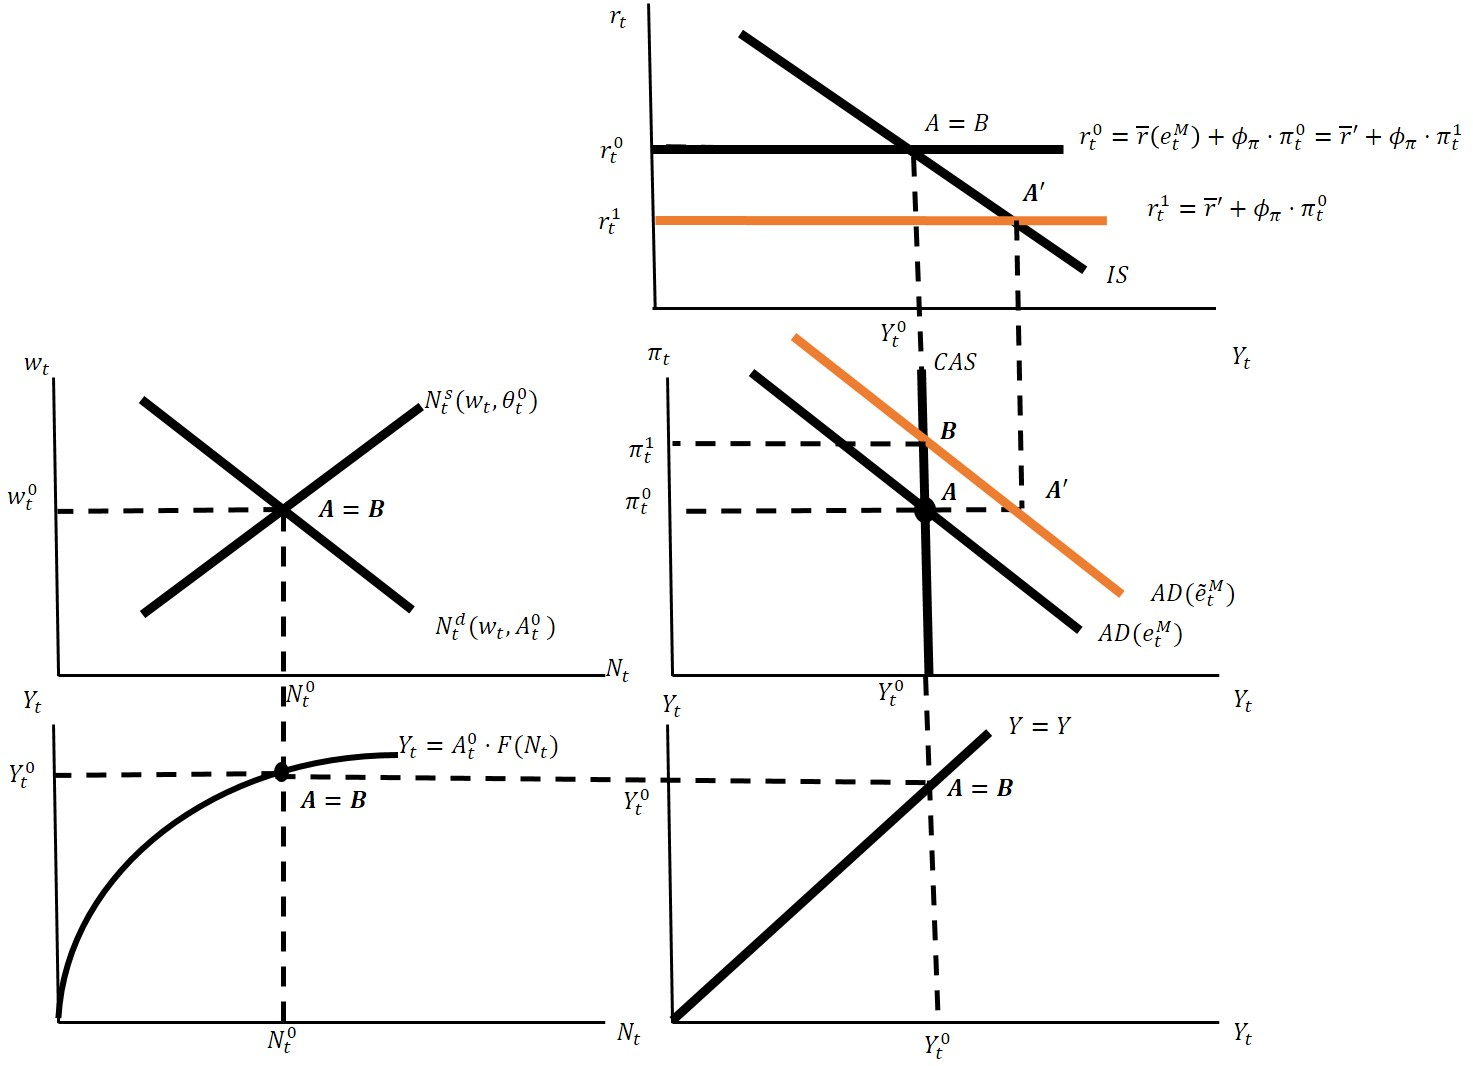
\includegraphics[width=\linewidth]{figADAS2.jpg}
\end{column}
\begin{column}{0.38\textwidth}
\small
\begin{itemize}
\item Monetary easing shifts AD right (for each $P$, higher $Y$).
\item In the IS--LM derivation, this is $M\uparrow$ or lower $i$ (higher real balances / lower real rate).
\item Equilibrium: $(Y,P)$ rise together in the short run.
\end{itemize}
\end{column}
\end{columns}
\end{frame}

%------------------------------------------------
\begin{frame}{Supply contraction: stagflation in one line}
\begin{columns}
\begin{column}{0.62\textwidth}
\centering
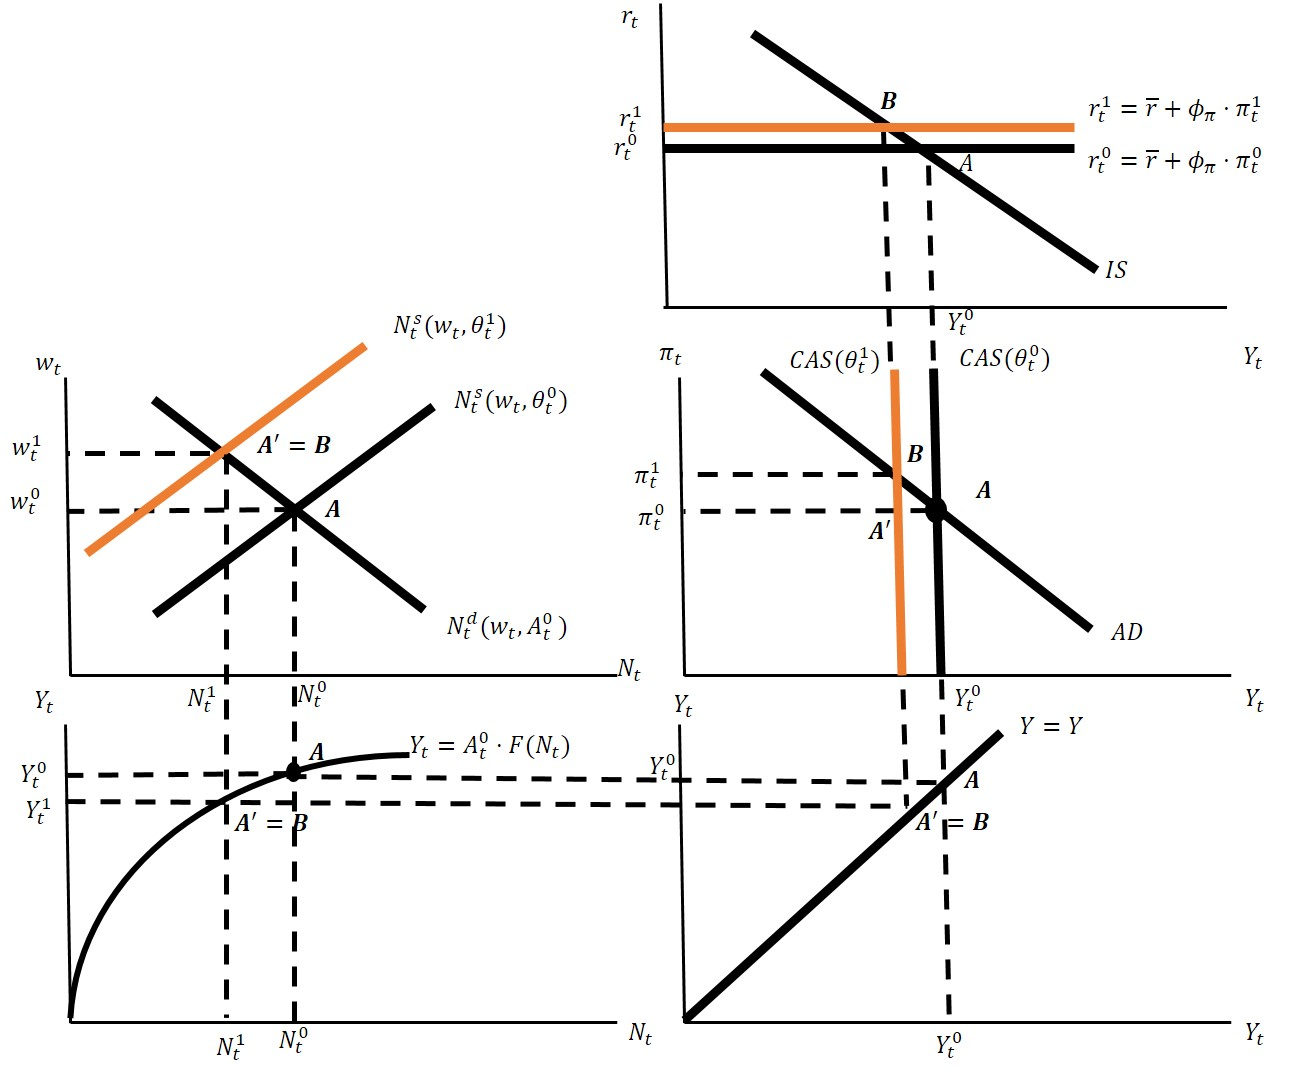
\includegraphics[width=\linewidth]{figADAS3.jpg}
\end{column}
\begin{column}{0.38\textwidth}
\small
\begin{itemize}
\item Supply contraction means $y^{FE}\downarrow$ or AS shifts up/left.
\item In the solved expression: if $y^{FE}$ falls, $p$ rises.
\item But lower $y^{FE}$ also pushes output down.
\end{itemize}
\end{column}
\end{columns}
\end{frame}

%------------------------------------------------
\begin{frame}{Medium run: expected price level catches up}
\begin{columns}
\begin{column}{0.62\textwidth}
\centering
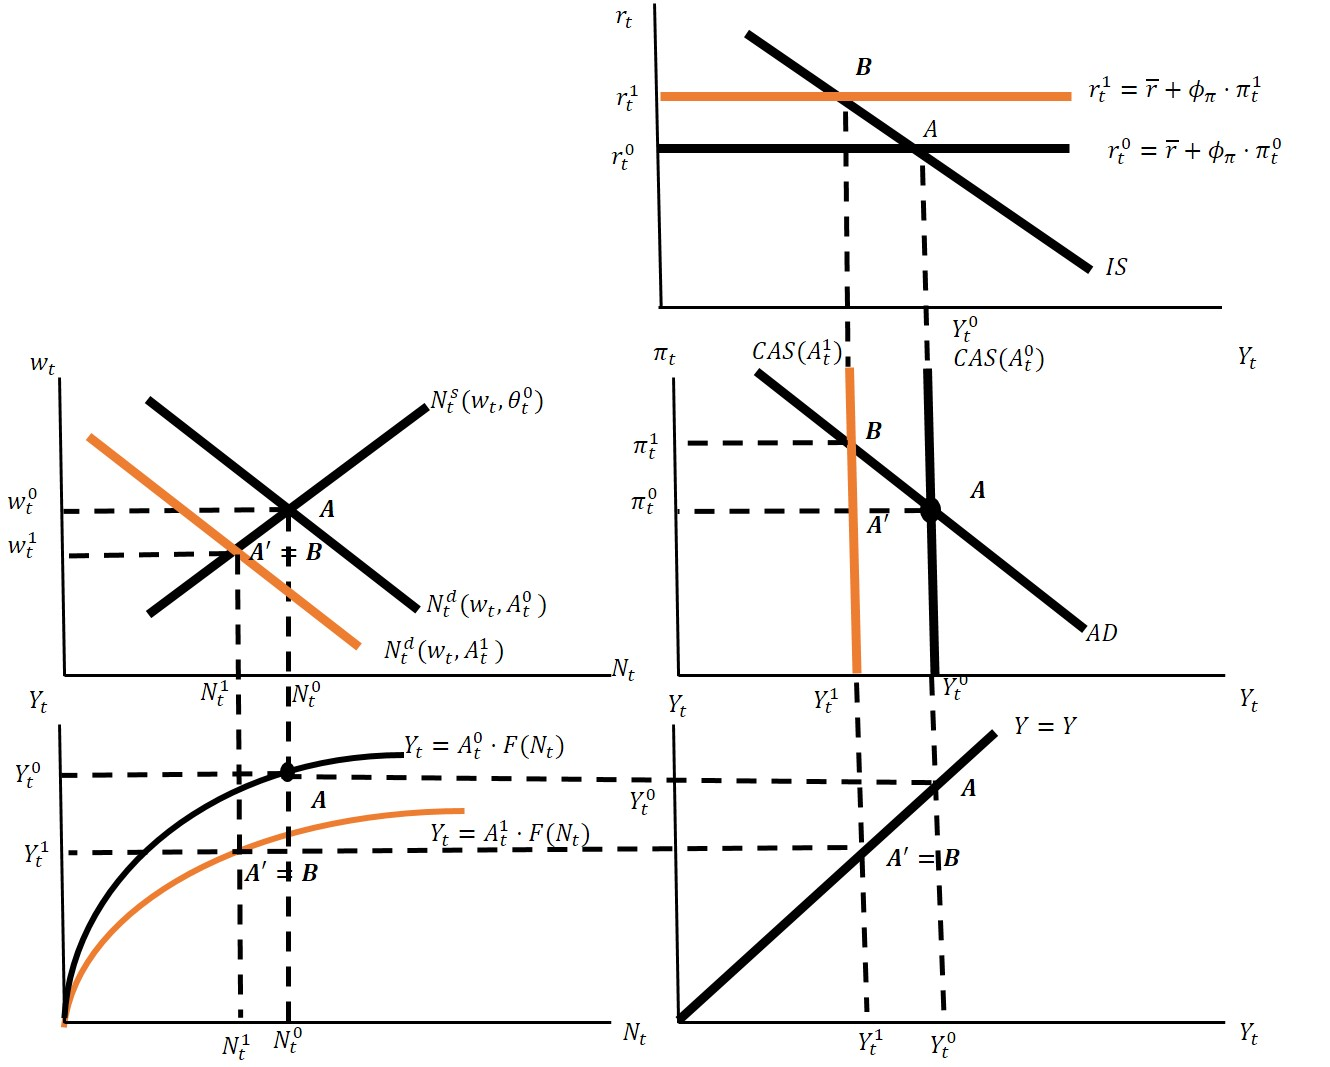
\includegraphics[width=\linewidth]{figADAS4.jpg}
\end{column}
\begin{column}{0.38\textwidth}
\small
\begin{itemize}
\item SRAS depends on $p^e$. When $p^e$ updates, SRAS shifts.
\item Medium-run logic: $p^e \uparrow$ until output returns to $y^{FE}$.
\item This is the bridge to next lecture: specify how $p^e$ evolves $\Rightarrow$ expected inflation.
\end{itemize}
\end{column}
\end{columns}
\end{frame}

%------------------------------------------------
\section[Summary]{One-page summary}

%------------------------------------------------
\begin{frame}{Cheat sheet: what each symbol means in the math AD--AS}
\small
\begin{itemize}
\item \textbf{Demand side (AD):} $y=\bar{y}_D-\phi p$ \quad (downward in $p$)
\begin{itemize}
\item $\bar{y}_D$ collects \emph{demand shifters}: $G$, taxes, wealth/optimism, monetary stance ($M$, $i$), etc.
\end{itemize}
\item \textbf{Supply side (SRAS):} $p=p^e+\lambda(y-y^{FE})$ \quad (upward in $y$)
\begin{itemize}
\item $y^{FE}$ is potential output from the RBC supply block (technology, labor, capital).
\item $p^e$ is the expected price level; updating $p^e$ shifts SRAS over time.
\end{itemize}
\item \textbf{Unemployment link:} $u-u^n\approx-\gamma x$ \quad (Okun).
\end{itemize}
\end{frame}

%------------------------------------------------
\begin{frame}{Next lecture (without naming ``Old Keynesian'' yet)}
\begin{itemize}
\item Replace $p^e$ with a rule for expected inflation (how expectations are formed).
\item Replace the level-form SRAS with an inflation form (Phillips curve language).
\item Introduce central bank practice: inflation targeting, Taylor rules, and how a policy rule shifts AD.
\end{itemize}
\end{frame}

\end{document}
